\documentclass[a4paper]{article}
\usepackage[a4paper,margin=0mm]{geometry}
\usepackage{fontspec}
\usepackage{unicode-math}
\usepackage{tikz}
\usetikzlibrary{fit,calc,positioning}
\usepackage[table]{xcolor}
\usepackage[absolute]{textpos}
\usepackage{array}

\setmainfont{Libertinus Serif}
\setsansfont{Libertinus Sans}
\setmathfont{Libertinus Math}

\definecolor{accent}{HTML}{F46530}
\definecolor{badge}{HTML}{FFBDA5}
\definecolor{ink}{HTML}{2A2E30}

\setlength{\TPHorizModule}{1mm}
\setlength{\TPVertModule}{1mm}
\setlength{\parindent}{0pt}
\pagestyle{empty}

\newcommand{\topicheader}[2]{%
\begin{textblock*}{194mm}(16mm,10mm)
\begin{tikzpicture}
\node[fill=accent,text=white,font=\sffamily\bfseries\fontsize{13}{13}\selectfont,
      minimum width=9mm,minimum height=9mm,inner sep=0pt] at (4.5mm,-4.5mm) {#1};
\node[font=\sffamily\bfseries\fontsize{15}{16}\selectfont,text=ink,anchor=west] at (12mm,-4.5mm) {#2};
\end{tikzpicture}
\end{textblock*}
\begin{textblock*}{194mm}(16mm,22.5mm)

\begin{tikzpicture}
\fill[accent] (0,0) rectangle (194mm,0.5mm);
\end{tikzpicture}
\end{textblock*}
}

\newcommand{\pagekicker}[1]{%
\begin{textblock*}{100mm}(16mm,25.5mm)
\begin{tikzpicture}
\node[fill=ink,text=white,font=\sffamily\bfseries\fontsize{8}{8}\selectfont,
      inner sep=2.2pt,rounded corners=1pt] {\MakeUppercase{#1}};
\end{tikzpicture}
\end{textblock*}
}

\newcommand{\pagefooter}[1]{%
\begin{textblock*}{194mm}(8mm,286.41mm)
  
\begin{tikzpicture}
    \fill[accent] (0,0) rectangle (194mm,0.6mm);
  \end{tikzpicture}
\end{textblock*}
\begin{textblock*}{63.59mm}(8mm,288.27mm)
  {\sffamily\bfseries\color{accent}\fontsize{13}{16}\selectfont SAT 1200+}
\end{textblock*}
\begin{textblock*}{10mm}(188mm,288.27mm)
  \centering{\sffamily\color{accent}\fontsize{14}{16}\selectfont #1}
\end{textblock*}
}

% ---- Card background: absolutely positioned, #1=x #2=y #3=width(mm) #4=height(mm) ----
\newcommand{\cardbg}[4]{%
\begin{textblock*}{#3mm}(#1mm,#2mm)
\begin{tikzpicture}
\fill[badge!22,rounded corners=3mm] (0,0) rectangle (#3mm,-#4mm);
\end{tikzpicture}
\end{textblock*}%
}

% ---- Pill label: absolutely positioned, #1=x #2=y #3=text ----
\newcommand{\pill}[3]{%
\begin{textblock*}{160mm}(#1mm,#2mm)
\begin{tikzpicture}
\node[fill=accent,text=white,anchor=north west,font=\sffamily\bfseries\fontsize{10}{10}\selectfont,
      rounded corners=8pt,inner xsep=5mm,inner ysep=1.8mm] at (0,0) {QOIDA ~\textperiodcentered~ #3};
\end{tikzpicture}
\end{textblock*}%
}

\arrayrulecolor{accent}
\setlength{\arrayrulewidth}{0.7pt}
\renewcommand{\arraystretch}{1.5}

\begin{document}

\topicheader{1}{Asosiy arifmetika va amallar tartibi}
\pagekicker{Formula sheet}
\pagefooter{7}
\mbox{}%

% ================= CARD 1: Amal nomlari (y: 33-93) =================
\cardbg{16}{33}{178}{60}
\pill{26}{36}{Amal nomlari}

\begin{textblock*}{158mm}(26mm,47mm)
{\fontsize{11}{14}\selectfont
\begin{tabular}{|>{\centering\arraybackslash}p{14mm}|p{40mm}|p{40mm}|p{40mm}|}
\hline
\rowcolor{accent}
{\color{white}\textbf{Belgi}} & {\color{white}\textbf{Amal}} & {\color{white}\textbf{Natija nomi}} & {\color{white}\textbf{English}} \\ \hline
$+$ & Qo'shish & Yig'indi & Sum \\ \hline
$-$ & Ayirish & Ayirma & Difference \\ \hline
$\times$ / $ab$ & Ko'paytirish & Ko'paytma & Product \\ \hline
$\dfrac{a}{b}$ & Bo'lish & Bo'linma & Quotient \\ \hline
\end{tabular}}
\end{textblock*}

% ================= CARD 2: Bajarish tartibi (y: 95-203) =================
\cardbg{16}{95}{178}{108}
\pill{26}{98}{Bajarish tartibi}

\begin{textblock*}{158mm}(26mm,109mm)
{\fontsize{11}{14}\selectfont\color{ink}
Har bir amal o'z bosqichiga ega. Bitta misolda barcha to'rt bosqich ketma-ket qanday ishlashini ko'ring:}
\end{textblock*}

\begin{textblock*}{158mm}(26mm,122mm)

\begin{tikzpicture}
\foreach \i/\x/\lbl in {1/0/{Qavs},2/40/{Daraja{\,/\,}Ildiz},3/80/{$\times$\ $\div$},4/118/{$+$\ $-$}}{
  \node[fill=accent,rounded corners=1.5pt,minimum height=7mm,minimum width=36mm,
        font=\sffamily\bfseries\fontsize{8.5}{9}\selectfont,text=white,align=center]
        at (\x mm+18mm,0) {\i.~\lbl};
}
\end{tikzpicture}
\end{textblock*}

\begin{textblock*}{158mm}(26mm,136mm)
\begin{tikzpicture}[every node/.style={font=\fontsize{13}{13}\selectfont}]
\node[anchor=west] (l0) at (0,0) {$5+2\times\underline{(8-3)}^2\div5$};
\node[anchor=west,font=\sffamily\bfseries\scriptsize,text=accent] at (82mm,0) {$\leftarrow$ 1. qavs};

\node[anchor=west] (l1) at (0,-10mm) {$5+2\times\underline{5^2}\div5$};
\node[anchor=west,font=\sffamily\bfseries\scriptsize,text=accent] at (82mm,-10mm) {$\leftarrow$ 2. daraja};

\node[anchor=west] (l2) at (0,-20mm) {$5+\underline{2\times25\div5}$};
\node[anchor=west,font=\sffamily\bfseries\scriptsize,text=accent] at (82mm,-20mm) {$\leftarrow$ 3. $\times\div$ (chapdan o'ngga)};

\node[anchor=west] (l3) at (0,-30mm) {$\underline{5+10}$};
\node[anchor=west,font=\sffamily\bfseries\scriptsize,text=accent] at (82mm,-30mm) {$\leftarrow$ 4. $+\,-$};

\node[anchor=west,font=\sffamily\bfseries\fontsize{14}{14}\selectfont,text=accent] (l4) at (0,-41mm) {$=15$};

\foreach \y in {-3,-13,-23,-33}{
  \draw[accent,->,line width=1pt] (6mm,\y mm) -- (6mm,\y mm -4mm);
}
\end{tikzpicture}
\end{textblock*}

\begin{textblock*}{178mm}(16mm,206mm)
{\fontsize{8.5}{10}\selectfont\color{black!55}\itshape 1-rasm.\ Bitta ifodaning to'rtala bosqich bo'yicha ketma-ket soddalashuvi.}
\end{textblock*}

% ================= CARD 3: Kasr chizig'i = qavs (y: 214-272, left half) =================
\cardbg{16}{214}{85}{58}
\pill{22}{217}{Kasr = qavs}

\begin{textblock*}{85mm}(16mm,230mm)
\begin{center}
\begin{tikzpicture}
\node[font=\fontsize{14}{14}\selectfont] (num) at (0,0) {$3+5$};
\node[font=\fontsize{14}{14}\selectfont] (den) at (0,-9mm) {$2\times2$};
\draw[ink,line width=0.7pt] (-9mm,-4.5mm) -- (9mm,-4.5mm);
\node[draw=accent,dashed,line width=0.9pt,rounded corners=1pt,fit=(num),inner sep=1.3mm] {};
\node[draw=accent,dashed,line width=0.9pt,rounded corners=1pt,fit=(den),inner sep=1.3mm] {};
\node[font=\sffamily\bfseries\fontsize{12}{12}\selectfont,text=accent] at (0,-17mm) {$=\dfrac{8}{4}=2$};
\end{tikzpicture}
\end{center}
\end{textblock*}

\begin{textblock*}{75mm}(20mm,260mm)
{\fontsize{8.5}{10}\selectfont\color{black!60}\itshape Yuqori va pastki qism -- har biri alohida qavsdagidek hisoblanadi.}
\end{textblock*}

% ================= CARD 4: Modul belgisi = qavs (y: 214-272, right half) =================
\cardbg{109}{214}{85}{58}
\pill{115}{217}{Modul = qavs}

\begin{textblock*}{85mm}(109mm,230mm)
\begin{center}
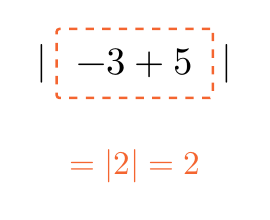
\begin{tikzpicture}
\node[font=\fontsize{14}{14}\selectfont] (bar1) at (0,0) {$|$};
\node[font=\fontsize{14}{14}\selectfont,right=1.2mm of bar1] (mid) {$-3+5$};
\node[font=\fontsize{14}{14}\selectfont,right=1.2mm of mid] (bar2) {$|$};
\node[draw=accent,dashed,line width=0.9pt,rounded corners=1pt,fit=(mid),inner sep=1.3mm] {};
\node[font=\sffamily\bfseries\fontsize{12}{12}\selectfont,text=accent] at ($(mid)+(0,-13mm)$) {$=|2|=2$};
\end{tikzpicture}
\end{center}
\end{textblock*}

\begin{textblock*}{75mm}(113mm,260mm)
{\fontsize{8.5}{10}\selectfont\color{black!60}\itshape Ichidagi amal avval, keyin natija musbat qilinadi.}
\end{textblock*}

\end{document}
